\documentclass[journal]{IEEEtran}
\usepackage{graphicx}

\begin{document}

\title{A performance based evaluation of ARMv8-A 32 bit and 64 bit execution}
\author{Dinesh K B, Radhish A, Anish N}

\maketitle

\begin{abstract}
In this paper we explore the raw performance of ARM32-bit versus ARM64-bit.  We use open source test suites on a Rasberry pi 3 board which uses A-53 processor, and compared the results.  The test suites were compiled with ARMv8-A architecture for both 32-bit and 64-bit, the details are provided later in this paper.  Our results shows that "the performance of 32-bit applications are comparible with 64-bit applications".  We also discuss the implications of our performance results and whether there is a need for porting the legacy 32-bit applications to 64-bit architecture.
\end{abstract}

\section{Introduction}
With over 86 billion ARM processors sold of 2016, ARM processors dominate the entire embedded space due to their high performance and low power requirements.  ARMv7-A is a 32 bit instruction set architecture, used in previous generation of ARM processor cores.  ARMv8-A, which was announced in Oct-2011, represents a major change to ARM architecture.  This adds an optional 64 bit architecture, referred as "AArch64". ARM's new 64 bit architecture is fully backward compatible with its 32 bit architecture (ARMv7-A). This means a 64 bit OS running on this processor can execute 32bit ARMv7-A binaries.  ARMv8-A 64-bit processors has been adopted by all the industry giants like Apple (A7), Samsung, Qualcomm and MediaTek etc.  Since all the 32 bit binaries can be executed on the ARMv8-A processors as is, this had made the adoption faster.  In this paper we have attempted to find out whether porting of 32 bit user applications to "AArch64" is really required, and whether there are any performance benefits in the doing this on "Raspberry pi 3 " board.

\section{Technical Overview}

\subsection{ARM Cortex-A53 processor}
The Cortex-A53 processor in Raspberry Pi 3, is a mid-range, low-power processor with four cores, each with an L1 cache subsystem. The Cortex-A53 processor is an extremely power efficient procesor capable of supporting 32-bit and 64-bit mode.
The Cortex-A53 processor has following features:
\begin{itemize}
	\item In-order, eight stage pipeline.
	\item Lower power consumption from the use of hierarchical clock gating, power domains, and advanced retention modes.
	\item Increased dual-issue capability from duplication of execution resources and dual instruction decoders.
	\item Power-optimized L2 cache design delivers lower latency and balances performance with efficiency.
\end{itemize}

\subsection{AARch64}
The ARM architecture is a Reduced Instruction Set Computer (RISC) architecture. ARMv8 is the latest version of ARM architecture.  An important feature of ARMv8 is that it supports two execution states AArch64 (64bit execution state) and AArch32 (32bit excution state).  AArch32 is compatible with ARMv7 architecture (pure 32bit architecture).  ARMv7-A Large Physical Address Extensions (LPAE), which provide 32 bit virtual address for 40 bit physical addressing, is supported in AArch32.

In AArch64 this is extended to provide 64 bit virtual addressing for 48 bit physical addressing.  Both AArch32 and AArch64 are 32 bit fixed length instruction set.  The AARch64 instruction set has been designed from scratch.  It operates on 64-bit or 32-bit data types and registers.  Neon now supports double-precision floating point and hardware divide support is included.  AArch64 doesnot support the shift and rotate operations in data processing instructions,  but it is still possible to shift, rotate the second operand.

\subsection{Register Set in AARch64}
AArch64 has 31 general purpose registers, all 64 bit.  These registers can be accessed by most instructions as 64 bit double words or as 32bit words.  All the registers can be accessed as 64-bit registers x0 - x30 or 32-bit sub registers w0 - w30.  If a register is written as 32-bit word, then the top half of the register is cleared.  All the base pointer registers are 64 bit to support 64 bit virtual addressing.  There are 32 registers for SIMD and Floating Point, all 128 bit wide.  These registers map differently than the earlier ARM architectures. Each AArch64 64-bit general-purpose register (X0-X30) also has a 32-bit (W0-W30) form.

\begin{figure}[h]
	\centering
    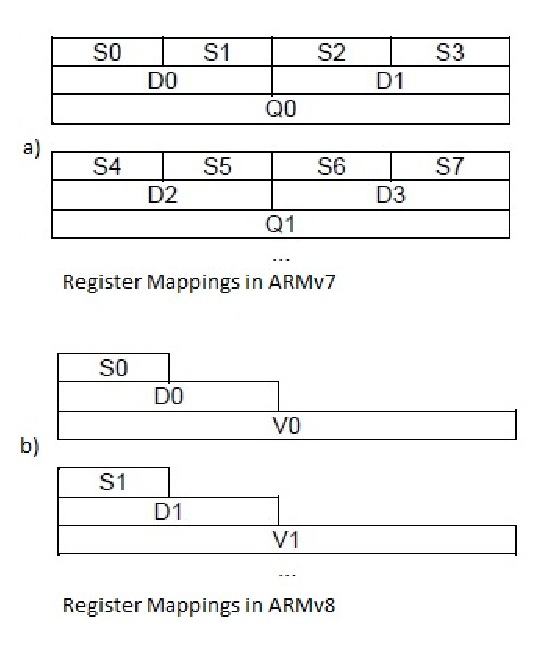
\includegraphics[width=3.0in]{./figures/reg.eps}
    \caption{Register mappings in ARMv7 and ARMv8.}
    \label{fig:Regfig}
\end{figure}

In earlier ARM architectures, the register set looked as shown in Fig \ref{fig:Regfig}(a). In AArch64, the register mapping has changed as shown in Fig \ref{fig:Regfig}(b).
The Program Counter (PC) can't be read or modified directly, unlike the other general registers.

\subsection{Execution States in ARMv8-A}
A fully populated ARMv8-A supports both AArch32 and AArch64 execution states. The transition between two states happens through exception boundary.  This is different than in ARMv7 where execution state changes from 32 bit instructions to 16 bit thumb instructions through interworking branch instruction(e.g. BLX). While taking or returning an exception, the execution state can change from 32 bit to 64 bit or vice versa.

\subsection{Execution Levels in AArch64}
The ARMv8 exception model defines Exception levels EL3-EL0, where EL0 is the least privileged and EL3 is the most privileged, in the order of increasing privileged levels. The execution levels are explained below, and in Fig \ref{fig:Execpfig}.

\begin{figure}[b!]
	\centering
    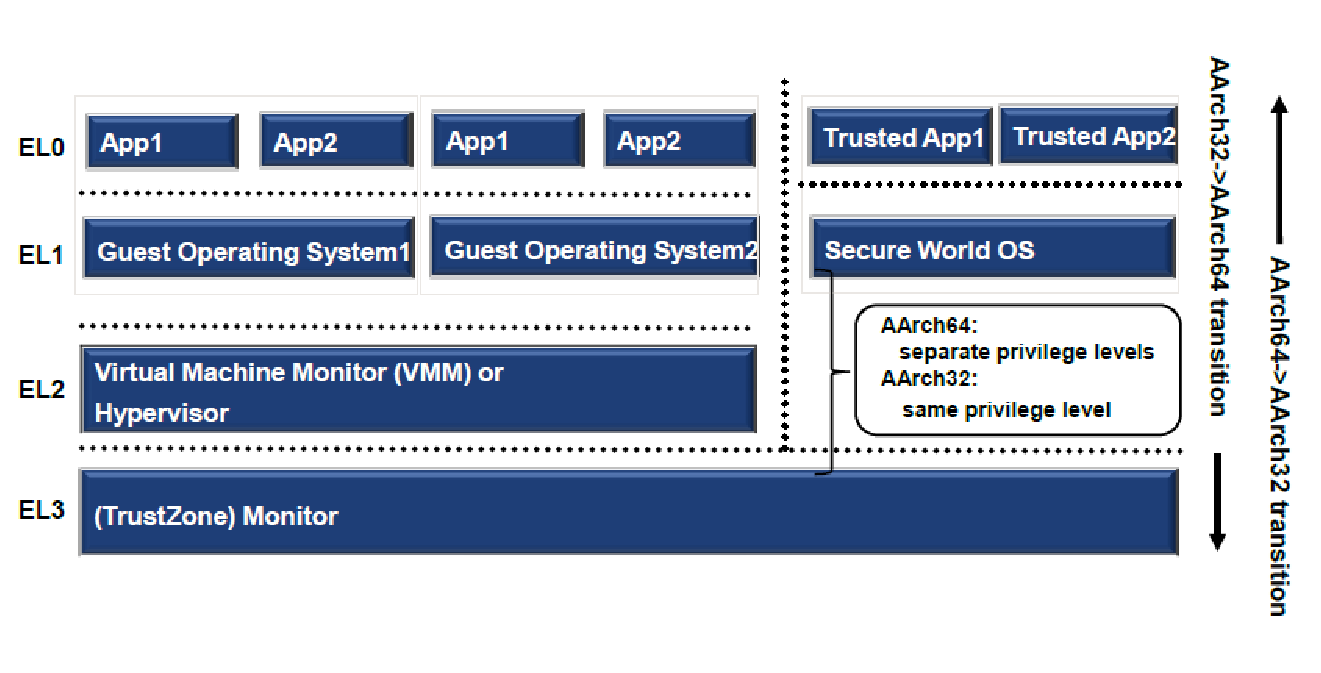
\includegraphics[width=7.0in]{./figures/exceptionLevels.eps}
    \caption{ARMv8 Exception Model.}
    \label{fig:Execpfig}
\end{figure}



\begin{itemize}
	\item EL0: Unprivileged execution. All user applications run in this level.
	\item EL1: Privileged level. OS Kernels typically run in this level.
	\item EL2: Provides support for processor virtualization (Hypervisor).
	\item EL3: Provides support for a Secure State.
\end{itemize}
Exceptions can be taken to the same or a higher exception level. There are different Vector Base Address Registers for EL1, EL2, EL3.


\subsection{Subsection Heading Here}
Write your subsection text here.

\section{Conclusion}
Write your conclusion here.

\section{References}
[1] Shore, Chris, July 2014. Porting to 64-bit ARM.
[2] http://infocenter.arm.com 

\end{document}
